% ---------------------------------------------------------------------------
\section{Commonality in empirical networks}
\label{sec:commonality}
% ---------------------------------------------------------------------------

The premise of the method is local: two adjacent nodes whose neighbourhoods largely
coincide belong, more often than not, to a common community. We test it on four
networks with recorded group memberships (Table~\ref{tab:data}): Zachary's karate
club~\cite{zachary1977information}, with its two post-split factions, and the DBLP
co-authorship, Amazon co-purchasing and YouTube friendship networks, whose ground-truth
groups (publication venues, product categories and user-created groups) come from the
Stanford Network Analysis Project (SNAP)~\cite{yang2015defining}.

\subsection{Unlabelled nodes and degree}

The SNAP networks label only part of their nodes: 82\% in DBLP, 95\% in Amazon and
4.6\% in YouTube. Counting pairs with an unlabelled node as pairs in different groups,
as the first author's earlier analysis did~\cite{deinega2023thesis},
is the standard pitfall of learning from positive and unlabelled
data~\cite{elkan2008learning}; on DBLP it reverses the conclusion, the area under the
ROC curve (AUC) falling to $0.41$, below chance. We therefore classify every edge as
\emph{inner} (both endpoints labelled and sharing a group), \emph{outer} (both labelled,
sharing none) or \emph{unlabelled}, and compare inner with outer only. ``Outer'' means
no \emph{recorded} shared group, and metadata need not coincide with structural
communities~\cite{peel2017ground,hric2014community}: the analysis tests a tendency, not
a classifier. With this correction commonality separates the classes on all four
networks, with AUCs of $0.82$, $0.62$, $0.60$ and $0.61$ in the order above
(Supplemental Material~\cite{supplement}, Fig.~\ref{fig:S-realcommonality}).

Jaccard commonality is capped by the degree ratio of the pair,
$J(u,v)\le (d_{\min}+1)/(d_{\max}+1)$, so edges incident to hubs have low $J$ whatever
their community structure, while degree also correlates with how labels were assigned.
Within strata of the larger endpoint degree the separation persists at every degree
[Fig.~\ref{fig:realcommonality}(a)]: the stratum AUCs range from $0.75$ to $0.87$ in
DBLP, all above the pooled $0.62$, and lie between $0.58$ and $0.67$ in Amazon and
between $0.53$ and $0.67$ in YouTube.

\subsection{Commonality is a family of functions}

Jaccard is one of many overlap scores catalogued for link
prediction~\cite{leicht2006vertex,zhou2009predicting,lu2011link}. With
$I=|N[u]\cap N[v]|$ and $U=|N[u]\cup N[v]|$ we compare eight (defined with
Fig.~\ref{fig:realfamily}): $I$, Jaccard $I/U$, $I^2/U$, $I/U^{1/2}$, the
cosine~\cite{salton1983introduction}, the hub-promoted $I/\min$ (after Ravasz
\emph{et al.}~\cite{ravasz2002hierarchical}) and hub-depressed $I/\max$, and resource
allocation (RA). Within
strata of both endpoint degrees every one separates inner from outer edges on the three SNAP networks
[Fig.~\ref{fig:realcommonality}(b)], and the overlap-based scores perform alike (DBLP
AUC $0.81$--$0.85$, Amazon $0.60$--$0.62$, YouTube $0.60$--$0.63$): at fixed endpoint
degrees each is a monotone function of $I$. They differ on pairs of \emph{different}
degrees, which a single global threshold must compare.
Pooled over all edges, no function is best everywhere: $I$ leads on DBLP ($0.78$,
against $0.62$ for Jaccard) but falls below chance on YouTube ($0.47$), where hubs
dominate, and $I/\min$ leads on the other three networks ($0.89$, $0.62$, $0.69$).
HyperCommon takes any member, the appropriate one depending on the network
(Sec.~\ref{sec:discussion}); unless stated otherwise we use Jaccard, the similarity of
link communities~\cite{ahn2010link}.

\subsection{From pairs to triples}

HyperCommon requires all three pairs of a wedge to pass the threshold, including the
pair that is not an edge. On unique labelled triples, call a triple \emph{pure} when one
recorded group contains all three nodes, and compare the \emph{pair rule}, which tests
only the edges of the triple (as in the two-test ablation of Sec.~\ref{sec:protocol}),
with the \emph{triple rule}, which also tests the non-adjacent pair of an open wedge. At
equal recall from $0.1$ to $0.4$ the triple rule is the more precise on all three SNAP
networks, with 95\% intervals of the difference that exclude zero
[Fig.~\ref{fig:realcommonality}(c)]; at recall $0.2$, $81\%$ of pair-admitted triples
are pure against $93\%$ of triple-admitted ones in DBLP. Beyond recall $\approx0.5$,
where most wedges are admitted, the pair rule is the more precise on DBLP
(Fig.~\ref{fig:realtriples}).
Section~\ref{sec:results} tests the third test and the admission of open wedges on the
final communities.

\begin{figure*}[t]
  \centering
  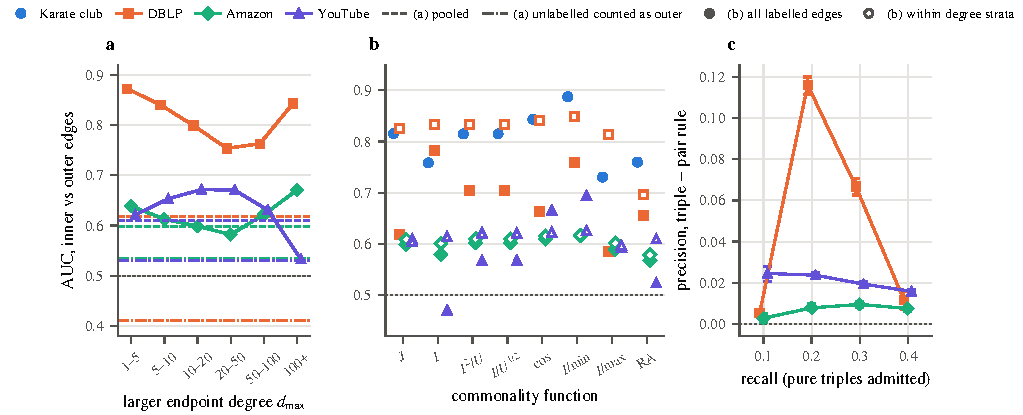
\includegraphics[width=\textwidth]{figures/fig_commonality.pdf}
  \caption{Commonality in networks with recorded memberships. (a)~AUC of
  closed-neighbourhood Jaccard for inner against outer edges within strata of $d_{\max}$
  (points), pooled (dashed), and with unlabelled edges counted as outer (dash-dotted), as
  in Ref.~\cite{deinega2023thesis}; the karate club is too small to stratify. (b)~AUC of
  eight functions over all labelled edges (filled) and within strata of both endpoint
  degrees (open). (c)~Precision of the triple minus the pair rule at equal recall, with
  95\% intervals from resampling the triples.}
  \label{fig:realcommonality}
\end{figure*}
